% Options for packages loaded elsewhere
\PassOptionsToPackage{unicode}{hyperref}
\PassOptionsToPackage{hyphens}{url}
\PassOptionsToPackage{dvipsnames,svgnames,x11names}{xcolor}
%
\documentclass[
  letterpaper,
  DIV=11,
  numbers=noendperiod]{scrartcl}

\usepackage{amsmath,amssymb}
\usepackage{lmodern}
\usepackage{iftex}
\ifPDFTeX
  \usepackage[T1]{fontenc}
  \usepackage[utf8]{inputenc}
  \usepackage{textcomp} % provide euro and other symbols
\else % if luatex or xetex
  \usepackage{unicode-math}
  \defaultfontfeatures{Scale=MatchLowercase}
  \defaultfontfeatures[\rmfamily]{Ligatures=TeX,Scale=1}
\fi
% Use upquote if available, for straight quotes in verbatim environments
\IfFileExists{upquote.sty}{\usepackage{upquote}}{}
\IfFileExists{microtype.sty}{% use microtype if available
  \usepackage[]{microtype}
  \UseMicrotypeSet[protrusion]{basicmath} % disable protrusion for tt fonts
}{}
\makeatletter
\@ifundefined{KOMAClassName}{% if non-KOMA class
  \IfFileExists{parskip.sty}{%
    \usepackage{parskip}
  }{% else
    \setlength{\parindent}{0pt}
    \setlength{\parskip}{6pt plus 2pt minus 1pt}}
}{% if KOMA class
  \KOMAoptions{parskip=half}}
\makeatother
\usepackage{xcolor}
\setlength{\emergencystretch}{3em} % prevent overfull lines
\setcounter{secnumdepth}{5}
% Make \paragraph and \subparagraph free-standing
\ifx\paragraph\undefined\else
  \let\oldparagraph\paragraph
  \renewcommand{\paragraph}[1]{\oldparagraph{#1}\mbox{}}
\fi
\ifx\subparagraph\undefined\else
  \let\oldsubparagraph\subparagraph
  \renewcommand{\subparagraph}[1]{\oldsubparagraph{#1}\mbox{}}
\fi

\usepackage{color}
\usepackage{fancyvrb}
\newcommand{\VerbBar}{|}
\newcommand{\VERB}{\Verb[commandchars=\\\{\}]}
\DefineVerbatimEnvironment{Highlighting}{Verbatim}{commandchars=\\\{\}}
% Add ',fontsize=\small' for more characters per line
\usepackage{framed}
\definecolor{shadecolor}{RGB}{241,243,245}
\newenvironment{Shaded}{\begin{snugshade}}{\end{snugshade}}
\newcommand{\AlertTok}[1]{\textcolor[rgb]{0.68,0.00,0.00}{#1}}
\newcommand{\AnnotationTok}[1]{\textcolor[rgb]{0.37,0.37,0.37}{#1}}
\newcommand{\AttributeTok}[1]{\textcolor[rgb]{0.40,0.45,0.13}{#1}}
\newcommand{\BaseNTok}[1]{\textcolor[rgb]{0.68,0.00,0.00}{#1}}
\newcommand{\BuiltInTok}[1]{\textcolor[rgb]{0.00,0.23,0.31}{#1}}
\newcommand{\CharTok}[1]{\textcolor[rgb]{0.13,0.47,0.30}{#1}}
\newcommand{\CommentTok}[1]{\textcolor[rgb]{0.37,0.37,0.37}{#1}}
\newcommand{\CommentVarTok}[1]{\textcolor[rgb]{0.37,0.37,0.37}{\textit{#1}}}
\newcommand{\ConstantTok}[1]{\textcolor[rgb]{0.56,0.35,0.01}{#1}}
\newcommand{\ControlFlowTok}[1]{\textcolor[rgb]{0.00,0.23,0.31}{#1}}
\newcommand{\DataTypeTok}[1]{\textcolor[rgb]{0.68,0.00,0.00}{#1}}
\newcommand{\DecValTok}[1]{\textcolor[rgb]{0.68,0.00,0.00}{#1}}
\newcommand{\DocumentationTok}[1]{\textcolor[rgb]{0.37,0.37,0.37}{\textit{#1}}}
\newcommand{\ErrorTok}[1]{\textcolor[rgb]{0.68,0.00,0.00}{#1}}
\newcommand{\ExtensionTok}[1]{\textcolor[rgb]{0.00,0.23,0.31}{#1}}
\newcommand{\FloatTok}[1]{\textcolor[rgb]{0.68,0.00,0.00}{#1}}
\newcommand{\FunctionTok}[1]{\textcolor[rgb]{0.28,0.35,0.67}{#1}}
\newcommand{\ImportTok}[1]{\textcolor[rgb]{0.00,0.46,0.62}{#1}}
\newcommand{\InformationTok}[1]{\textcolor[rgb]{0.37,0.37,0.37}{#1}}
\newcommand{\KeywordTok}[1]{\textcolor[rgb]{0.00,0.23,0.31}{#1}}
\newcommand{\NormalTok}[1]{\textcolor[rgb]{0.00,0.23,0.31}{#1}}
\newcommand{\OperatorTok}[1]{\textcolor[rgb]{0.37,0.37,0.37}{#1}}
\newcommand{\OtherTok}[1]{\textcolor[rgb]{0.00,0.23,0.31}{#1}}
\newcommand{\PreprocessorTok}[1]{\textcolor[rgb]{0.68,0.00,0.00}{#1}}
\newcommand{\RegionMarkerTok}[1]{\textcolor[rgb]{0.00,0.23,0.31}{#1}}
\newcommand{\SpecialCharTok}[1]{\textcolor[rgb]{0.37,0.37,0.37}{#1}}
\newcommand{\SpecialStringTok}[1]{\textcolor[rgb]{0.13,0.47,0.30}{#1}}
\newcommand{\StringTok}[1]{\textcolor[rgb]{0.13,0.47,0.30}{#1}}
\newcommand{\VariableTok}[1]{\textcolor[rgb]{0.07,0.07,0.07}{#1}}
\newcommand{\VerbatimStringTok}[1]{\textcolor[rgb]{0.13,0.47,0.30}{#1}}
\newcommand{\WarningTok}[1]{\textcolor[rgb]{0.37,0.37,0.37}{\textit{#1}}}

\providecommand{\tightlist}{%
  \setlength{\itemsep}{0pt}\setlength{\parskip}{0pt}}\usepackage{longtable,booktabs,array}
\usepackage{calc} % for calculating minipage widths
% Correct order of tables after \paragraph or \subparagraph
\usepackage{etoolbox}
\makeatletter
\patchcmd\longtable{\par}{\if@noskipsec\mbox{}\fi\par}{}{}
\makeatother
% Allow footnotes in longtable head/foot
\IfFileExists{footnotehyper.sty}{\usepackage{footnotehyper}}{\usepackage{footnote}}
\makesavenoteenv{longtable}
\usepackage{graphicx}
\makeatletter
\def\maxwidth{\ifdim\Gin@nat@width>\linewidth\linewidth\else\Gin@nat@width\fi}
\def\maxheight{\ifdim\Gin@nat@height>\textheight\textheight\else\Gin@nat@height\fi}
\makeatother
% Scale images if necessary, so that they will not overflow the page
% margins by default, and it is still possible to overwrite the defaults
% using explicit options in \includegraphics[width, height, ...]{}
\setkeys{Gin}{width=\maxwidth,height=\maxheight,keepaspectratio}
% Set default figure placement to htbp
\makeatletter
\def\fps@figure{htbp}
\makeatother

\KOMAoption{captions}{tableheading}
\makeatletter
\makeatother
\makeatletter
\makeatother
\makeatletter
\@ifpackageloaded{caption}{}{\usepackage{caption}}
\AtBeginDocument{%
\ifdefined\contentsname
  \renewcommand*\contentsname{Table of contents}
\else
  \newcommand\contentsname{Table of contents}
\fi
\ifdefined\listfigurename
  \renewcommand*\listfigurename{List of Figures}
\else
  \newcommand\listfigurename{List of Figures}
\fi
\ifdefined\listtablename
  \renewcommand*\listtablename{List of Tables}
\else
  \newcommand\listtablename{List of Tables}
\fi
\ifdefined\figurename
  \renewcommand*\figurename{Figure}
\else
  \newcommand\figurename{Figure}
\fi
\ifdefined\tablename
  \renewcommand*\tablename{Table}
\else
  \newcommand\tablename{Table}
\fi
}
\@ifpackageloaded{float}{}{\usepackage{float}}
\floatstyle{ruled}
\@ifundefined{c@chapter}{\newfloat{codelisting}{h}{lop}}{\newfloat{codelisting}{h}{lop}[chapter]}
\floatname{codelisting}{Listing}
\newcommand*\listoflistings{\listof{codelisting}{List of Listings}}
\makeatother
\makeatletter
\@ifpackageloaded{caption}{}{\usepackage{caption}}
\@ifpackageloaded{subcaption}{}{\usepackage{subcaption}}
\makeatother
\makeatletter
\@ifpackageloaded{tcolorbox}{}{\usepackage[many]{tcolorbox}}
\makeatother
\makeatletter
\@ifundefined{shadecolor}{\definecolor{shadecolor}{rgb}{.97, .97, .97}}
\makeatother
\makeatletter
\makeatother
\ifLuaTeX
  \usepackage{selnolig}  % disable illegal ligatures
\fi
\IfFileExists{bookmark.sty}{\usepackage{bookmark}}{\usepackage{hyperref}}
\IfFileExists{xurl.sty}{\usepackage{xurl}}{} % add URL line breaks if available
\urlstyle{same} % disable monospaced font for URLs
\hypersetup{
  pdftitle={Demand of Football in European Leagues},
  pdfauthor={Matthew Wilcox},
  colorlinks=true,
  linkcolor={blue},
  filecolor={Maroon},
  citecolor={Blue},
  urlcolor={Blue},
  pdfcreator={LaTeX via pandoc}}

\title{Demand of Football in European Leagues}
\usepackage{etoolbox}
\makeatletter
\providecommand{\subtitle}[1]{% add subtitle to \maketitle
  \apptocmd{\@title}{\par {\large #1 \par}}{}{}
}
\makeatother
\subtitle{DATA 450 Capstone}
\author{Matthew Wilcox}
\date{}

\begin{document}
\maketitle
\ifdefined\Shaded\renewenvironment{Shaded}{\begin{tcolorbox}[interior hidden, enhanced, sharp corners, frame hidden, boxrule=0pt, breakable, borderline west={3pt}{0pt}{shadecolor}]}{\end{tcolorbox}}\fi

\hypertarget{introduction}{%
\section{Introduction}\label{introduction}}

Football (Soccer) is the most populat sport in the world. With an
estimated 3.5 billion fans world wide it is the most viewed sport in the
word {[}https://sportforbusiness.com/the-worlds-most-watched-sports/{]}.
Being such a popular sport, there is a large business and economy
surrounding the sport. Football teams need to be profitable to succeed.
These teams have 5 primary revenue sources. They are television money,
prize money, player transfers, sponsorships, and matchday
revenues{[}https://www.football-stadiums.co.uk/articles/how-do-football-clubs-make-money/{]}.
Out of all of these one of the most universial is matchday revenues.
Television, prize money, player transfers, and sponsorships can all vary
based on what level the team is at. Matchday revenues are much more
applicable at all levels of the game. Match day revenues are the profits
a team makes from people attending the game. This is from ticket,
consessions, and merchandise sales from attending a game. For many teams
this is the lifeblood of the club and what allows for the club to
survie.

The most important factor within match day revenues is the attendnace.
The amount of people that will attend a given match will greatly affect
the match day revenues. So understanding factors and being able to
predict the attendance for a given match is so important. If a club was
able to predict the amount of people that will attend a given match,
they could be better prepared for an individual match. Additionally if a
predicted match was predicted to have lower attendnace then desired from
the club, the club could market it differently or have special
promotions in an attempt to increase the attendance for that match.

What has been done here is an evaluation of factors that may impact the
attendance for an individual match. These factors are the day/time of
the match, betting odds for a match, and whom the away team is for any
given match. Additionally, in the end a random forest model was produced
to predict attendnace of matches based on these factors.

\begin{Shaded}
\begin{Highlighting}[]
\ImportTok{import}\NormalTok{ seaborn }\ImportTok{as}\NormalTok{ sns}
\ImportTok{from}\NormalTok{ sklearn.ensemble }\ImportTok{import}\NormalTok{ RandomForestRegressor}
\ImportTok{import}\NormalTok{ numpy }\ImportTok{as}\NormalTok{ np}
\ImportTok{import}\NormalTok{ matplotlib.pyplot }\ImportTok{as}\NormalTok{ plt}
\ImportTok{import}\NormalTok{ pandas }\ImportTok{as}\NormalTok{ pd}
\ImportTok{from}\NormalTok{ sklearn.preprocessing }\ImportTok{import}\NormalTok{ LabelEncoder}
\ImportTok{from}\NormalTok{ sklearn.model\_selection }\ImportTok{import}\NormalTok{ train\_test\_split}
\ImportTok{from}\NormalTok{ sklearn.metrics }\ImportTok{import}\NormalTok{ mean\_squared\_error}
\ImportTok{from}\NormalTok{ sklearn.metrics }\ImportTok{import}\NormalTok{ accuracy\_score, confusion\_matrix, classification\_report}
\ImportTok{from}\NormalTok{ sklearn }\ImportTok{import}\NormalTok{ metrics}
\ImportTok{from}\NormalTok{ sklearn.linear\_model }\ImportTok{import}\NormalTok{ LinearRegression}
\ImportTok{import}\NormalTok{ july}
\ImportTok{from}\NormalTok{ datetime }\ImportTok{import}\NormalTok{ datetime }\ImportTok{as}\NormalTok{ dt}
\ImportTok{from}\NormalTok{ jupyter\_dash }\ImportTok{import}\NormalTok{ JupyterDash}
\ImportTok{from}\NormalTok{ dash }\ImportTok{import}\NormalTok{ html, dcc, Input, Output}
\ImportTok{import}\NormalTok{ plotly.graph\_objects }\ImportTok{as}\NormalTok{ go}
\ImportTok{import}\NormalTok{ plotly.express }\ImportTok{as}\NormalTok{ px}
\end{Highlighting}
\end{Shaded}

\hypertarget{data-collection}{%
\section{Data Collection}\label{data-collection}}

The data used in this project was collected from two sources:
worldfootball.net and Football-data.co.uk. The data that was collected
from worldfootball.net was information on the match such as the names of
the teams, the time and date of the match, and most importantly the
attendnace for an individual match. This data was not already tabulated
so it was scraped from the website. This scrape occured on January 31st
2023. The data that was collected from Football-data.co.uk was primarily
betting information for each game. This data was already tabulated into
csv files however they were divided based upon the year and league. All
the files were downloaded on Febuary 3rd 2023.

The data that was collected was between 2010 and 2023. It consisted of
leagues from 11 countries being England, Scotland, Germany, Italy,
Spain, France, Netherlands, Belgium, Portugal, Turkey, and Greece. From
these Countries 21 leagues of data was collected.

\hypertarget{data-processing}{%
\section{Data Processing}\label{data-processing}}

All of the csv file's from Football-data.co.uk were combined togther
resulting in two datasets. One with all of the betting data and the
other with the attendance. These two datasets were to be combined on the
home team name, away team name, and the date/time of the game. However,
the two data sets had differnet naming structures for team names. For
example, the team Manchester City in one dataset would be identified as
``man\_city'' and in the other as ``manchester\_city''. With this
differenting structures and spellings of team names, a list of team
names was created for both datasets. These lists were than put through a
script that took a team from one list and compared the characters to
values in the other list. This was starting with one entire team and
slowly decreasing its size and observign that through the other team
list.

\begin{longtable}[]{@{}ll@{}}
\toprule()
Itteration & Results \\
\midrule()
\endhead
1 & man\_city \\
2 & man\_cit, an\_city \\
3 & man\_ci, an\_cit, n\_city \\
4 & man\_c, an\_ci, n\_cit, \_city \\
\bottomrule()
\end{longtable}

This is an example of how it would divide the name of one list up. It
would do this until the team list was broken up into single characters.
Then It would start with the largest length of a team name and look
through the other list for any results, It would then proceed through
the remaining potential names. What resulted is a list of potential
matching teams with the team with the most similar name at the top. Then
I would determine from the suggestion what was the matching team name.
Now that the two data sets had a matching naming of home and away teams,
the data sets were able to combine. The resulting data set had 79673
rows and 172 columns where each row was an individual match.

However more processing was needed. Although the intial dataset
collected data all the way to 2023, the range of the data was filterd to
only 2010 to 2019. This was to attribute to the COVID-19 pandemic.
During the pandemic attendance basically ceased to occur for matches.
Additionally some leagues cancelled the remaining matches for the
season. For those reasons the dataset is focused up untill that time.

Certain leagues were removed from the dataset for analysis . The Scotish
Divsiion 2 and Division 3 leagues as well as the Ethniki Katigoria,
which is the Greek top league, were removed. This is due to them having
several missing values for many variables. Some matches from a variety
of leagues had missing values for only betting variables. These matches
within leagues were used during the analysis of day/time and the impact
of the away team, however, were dropped from the dataset for analysis
betting data and in the modeling.

Lastly a few new variables were added. The first variable added was the
Season the match occured. Although leagues end on different dates on
different years the date selected for the season to switch was July
14th. Most leagues conclude in the begining of June and start back in
the begining fo August. July is predominantly used for international
games. Although there were a couple of matches that occured in July from
2010-2019, July 14th was the only date with zero matches played. So it
was used as the cutoff point.

The other variables were the mean and standard deviaiton of the home
team for that season and the z-score of that individual match. The mean
and standard deviation were just used to create to create the z-score
variable. The z-score is the standardization of the mathces attendance
in relation to the home team's average attendance for that particular
season.

\hypertarget{final-dataset}{%
\subsection{Final Dataset}\label{final-dataset}}

The resulting dataset that was used consisted fo 53,224 rowss and 34
columns. Here is a list of the variables used as well as their
description:

\begin{longtable}[]{@{}
  >{\raggedright\arraybackslash}p{(\columnwidth - 2\tabcolsep) * \real{0.5000}}
  >{\raggedright\arraybackslash}p{(\columnwidth - 2\tabcolsep) * \real{0.5000}}@{}}
\toprule()
\begin{minipage}[b]{\linewidth}\raggedright
Variable
\end{minipage} & \begin{minipage}[b]{\linewidth}\raggedright
Description
\end{minipage} \\
\midrule()
\endhead
home\_team & Name of Home team for na individual match \\
away\_team & Name of Away team for an individual match \\
raw\_attendance & Total number of people who attended an individual
match \\
division & The league the match took place in \\
B365H & Bet365 home team win odds \\
B365D & Bet 365 draw odds \\
B365A & Bet365 away team win odds \\
BWH & Bet\&Win home team win odds \\
BWD & Bet\&Win draw odds \\
BWA & Bet\&Win away team odds \\
WHH & William Hilll Home win Odds \\
WHD & William Hill Draw odds \\
WHA & William Hill Away win odds \\
VCH & VC Bet Home team win odds \\
VCD & VC bet draw odds \\
VCA & VC Bet away win odds \\
BbAv\textgreater2.5 & Bet Brain Average over 2.5 goals \\
BbAV\textless2.5 & Bet Brain Average under 2.5 goals \\
date\_time & Date and time of when a match occured \\
season & The season a match occured \\
mean\_attend & Average home team attednace for that season \\
std\_attend & Standard deviation of the home team attendance that
season \\
Standard\_attendance & The z-score of attendance for a match in relation
to the home team attednacne that season \\
\bottomrule()
\end{longtable}

\begin{Shaded}
\begin{Highlighting}[]
\NormalTok{total\_data }\OperatorTok{=}\NormalTok{ pd.read\_pickle(}\StringTok{\textquotesingle{}../data/final\_datasets/data\_standardized.pkl\textquotesingle{}}\NormalTok{)}
\NormalTok{total\_data.head()}
\end{Highlighting}
\end{Shaded}

\begin{verbatim}
C:\Users\Matthew Wilcox\AppData\Roaming\Python\Python310\site-packages\IPython\core\formatters.py:343: FutureWarning:

In future versions `DataFrame.to_latex` is expected to utilise the base implementation of `Styler.to_latex` for formatting and rendering. The arguments signature may therefore change. It is recommended instead to use `DataFrame.style.to_latex` which also contains additional functionality.
\end{verbatim}

\begin{tabular}{lllrrlllrlllrllrrlrrlrrrrrrrrrrrrrrrrrlrrrr}
\toprule
{} &          home\_team &                away\_team &  home\_score &  away\_score &        date &   time & day\_of\_week &  raw\_attendance &       stadium &    city &  country &  capacity &                                                url & division &  FTHG &  FTAG & FTR &  HTHG &  HTAG & HTR &  B365H &  B365D &  B365A &   BWH &   BWD &    BWA &   WHH &   WHD &   WHA &   VCH &  VCD &   VCA &  BbMx>2.5 &  BbAv>2.5 &  BbMx<2.5 &  BbAv<2.5 &  capacity\_filled &           date\_time &  season &   mean\_attend &  std\_attend &  standard\_attend \\
\midrule
0 &  tottenham\_hotspur &          manchester\_city &           0 &           0 &  2010-08-14 &  12:45 &    Saturday &           35928 &  Stadium News &  London &  England &   36284.0 &  https://www.worldfootball.net/venues/white-har... &       E0 &   0.0 &   0.0 &   D &   0.0 &   0.0 &   D &   2.40 &   3.30 &   3.00 &  2.35 &  3.30 &   2.85 &  2.38 &  3.25 &   3.0 &  2.30 &  3.4 &   3.1 &      2.03 &      1.91 &      1.95 &      1.84 &         0.990189 & 2010-08-14 12:45:00 &    2011 &  35892.894737 &  269.766338 &         0.130132 \\
1 &  tottenham\_hotspur &           wigan\_athletic &           0 &           1 &  2010-08-28 &  15:00 &    Saturday &           35101 &  Stadium News &  London &  England &   36284.0 &  https://www.worldfootball.net/venues/white-har... &       E0 &   0.0 &   1.0 &   A &   0.0 &   0.0 &   D &   1.25 &   5.75 &  13.00 &  1.22 &  5.75 &  11.50 &  1.25 &  5.50 &  12.0 &  1.25 &  6.0 &  13.0 &      1.55 &      1.50 &      2.63 &      2.48 &         0.967396 & 2010-08-28 15:00:00 &    2011 &  35892.894737 &  269.766338 &        -2.935484 \\
2 &  tottenham\_hotspur &  wolverhampton\_wanderers &           3 &           1 &  2010-09-18 &  15:00 &    Saturday &           35940 &  Stadium News &  London &  England &   36284.0 &  https://www.worldfootball.net/venues/white-har... &       E0 &   3.0 &   1.0 &   H &   0.0 &   1.0 &   A &   1.40 &   4.50 &   8.50 &  1.40 &  4.25 &   7.50 &  1.44 &  4.20 &   8.5 &  1.44 &  4.4 &   8.0 &      1.85 &      1.75 &      2.11 &      2.02 &         0.990519 & 2010-09-18 15:00:00 &    2011 &  35892.894737 &  269.766338 &         0.174615 \\
3 &  tottenham\_hotspur &               everton\_fc &           1 &           1 &  2010-10-23 &  12:45 &    Saturday &           35967 &  Stadium News &  London &  England &   36284.0 &  https://www.worldfootball.net/venues/white-har... &       E0 &   1.0 &   1.0 &   D &   1.0 &   1.0 &   D &   2.10 &   3.25 &   3.75 &  1.95 &  3.30 &   3.75 &  2.05 &  3.20 &   3.8 &  2.10 &  3.4 &   4.0 &      2.07 &      1.99 &      1.87 &      1.79 &         0.991263 & 2010-10-23 12:45:00 &    2011 &  35892.894737 &  269.766338 &         0.274702 \\
4 &  tottenham\_hotspur &           sunderland\_afc &           1 &           1 &  2010-09-11 &  20:00 &     Tuesday &           35843 &  Stadium News &  London &  England &   36284.0 &  https://www.worldfootball.net/venues/white-har... &       E0 &   1.0 &   1.0 &   D &   0.0 &   0.0 &   D &   1.53 &   4.00 &   6.50 &  1.48 &  4.00 &   6.50 &  1.57 &  3.80 &   6.0 &  1.57 &  4.0 &   7.0 &      1.90 &      1.80 &      2.06 &      1.97 &         0.987846 & 2010-09-11 20:00:00 &    2011 &  35892.894737 &  269.766338 &        -0.184955 \\
\bottomrule
\end{tabular}

\hypertarget{date-time}{%
\section{Date \& Time}\label{date-time}}

The first factor that will be evaluated is the date and time of
individual matches. There are multiple attributes to this that will be
viewed, from the day of the week, calendar date, and time of the match.

\begin{Shaded}
\begin{Highlighting}[]
\NormalTok{time\_df }\OperatorTok{=}\NormalTok{ total\_data[[}
    \StringTok{\textquotesingle{}date\textquotesingle{}}\NormalTok{, }\StringTok{\textquotesingle{}time\textquotesingle{}}\NormalTok{, }\StringTok{\textquotesingle{}day\_of\_week\textquotesingle{}}\NormalTok{, }\StringTok{\textquotesingle{}date\_time\textquotesingle{}}\NormalTok{, }\StringTok{\textquotesingle{}raw\_attendance\textquotesingle{}}\NormalTok{, }\StringTok{\textquotesingle{}capacity\_filled\textquotesingle{}}\NormalTok{, }\StringTok{\textquotesingle{}standard\_attend\textquotesingle{}}\NormalTok{, }\StringTok{\textquotesingle{}division\textquotesingle{}}
\NormalTok{]]}


\NormalTok{df\_grouped\_mean }\OperatorTok{=}\NormalTok{ time\_df.groupby(}\StringTok{\textquotesingle{}day\_of\_week\textquotesingle{}}\NormalTok{)[}\StringTok{\textquotesingle{}raw\_attendance\textquotesingle{}}\NormalTok{, }\StringTok{\textquotesingle{}capacity\_filled\textquotesingle{}}\NormalTok{, }\StringTok{\textquotesingle{}standard\_attend\textquotesingle{}}\NormalTok{].mean().reset\_index()}
\NormalTok{df\_grouped\_median }\OperatorTok{=}\NormalTok{ time\_df.groupby(}\StringTok{\textquotesingle{}day\_of\_week\textquotesingle{}}\NormalTok{)[}\StringTok{\textquotesingle{}raw\_attendance\textquotesingle{}}\NormalTok{, }\StringTok{\textquotesingle{}capacity\_filled\textquotesingle{}}\NormalTok{, }\StringTok{\textquotesingle{}standard\_attend\textquotesingle{}}\NormalTok{].median().reset\_index()}

\NormalTok{day\_categories }\OperatorTok{=}\NormalTok{ [}\StringTok{\textquotesingle{}Monday\textquotesingle{}}\NormalTok{, }\StringTok{\textquotesingle{}Tuesday\textquotesingle{}}\NormalTok{, }\StringTok{\textquotesingle{}Wednesday\textquotesingle{}}\NormalTok{, }\StringTok{\textquotesingle{}Thursday\textquotesingle{}}\NormalTok{, }\StringTok{\textquotesingle{}Friday\textquotesingle{}}\NormalTok{, }\StringTok{\textquotesingle{}Saturday\textquotesingle{}}\NormalTok{, }\StringTok{\textquotesingle{}Sunday\textquotesingle{}}\NormalTok{]}
\NormalTok{df\_grouped\_median[}\StringTok{\textquotesingle{}day\_of\_week\textquotesingle{}}\NormalTok{] }\OperatorTok{=}\NormalTok{ pd.Categorical(df\_grouped\_median[}\StringTok{\textquotesingle{}day\_of\_week\textquotesingle{}}\NormalTok{], categories}\OperatorTok{=}\NormalTok{ day\_categories)}
\NormalTok{df\_grouped\_median.sort\_values(by }\OperatorTok{=} \StringTok{\textquotesingle{}day\_of\_week\textquotesingle{}}\NormalTok{, inplace }\OperatorTok{=} \VariableTok{True}\NormalTok{)}
\end{Highlighting}
\end{Shaded}

\hypertarget{day-of-week}{%
\subsection{Day of Week}\label{day-of-week}}

First in Figure~\ref{fig-day_median_attend}, the average attendance for
matches are being viewed by the day of the week. What is significant
here is that it appears that wednesday and sunday has the highest
average attendance while Tuesday has the lowest. Wednesday being having
the highest average attendance is striking. Most would expect games on
the weekday games may have struggle to have high attendance

\begin{Shaded}
\begin{Highlighting}[]
\NormalTok{sns.barplot(data}\OperatorTok{=}\NormalTok{df\_grouped\_median, x }\OperatorTok{=} \StringTok{\textquotesingle{}day\_of\_week\textquotesingle{}}\NormalTok{, y }\OperatorTok{=} \StringTok{\textquotesingle{}raw\_attendance\textquotesingle{}}\NormalTok{).}\BuiltInTok{set}\NormalTok{(title }\OperatorTok{=}\StringTok{\textquotesingle{}Median  Attendance by Day of Week\textquotesingle{}}\NormalTok{)}
\NormalTok{plt.xticks(rotation}\OperatorTok{=}\DecValTok{90}\NormalTok{)}
\NormalTok{plt.xlabel(}\StringTok{\textquotesingle{}Day of the Week\textquotesingle{}}\NormalTok{)}
\NormalTok{plt.ylabel(}\StringTok{\textquotesingle{}Median Attendance\textquotesingle{}}\NormalTok{)}
\NormalTok{plt.show()}
\end{Highlighting}
\end{Shaded}

\begin{figure}[H]

{\centering 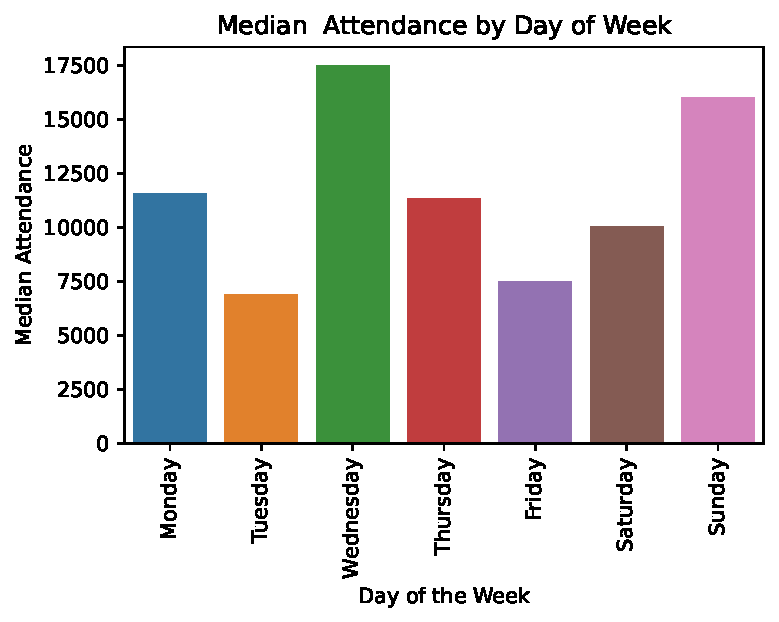
\includegraphics{Blog_post_files/figure-pdf/fig-day_median_attend-output-1.pdf}

}

\caption{\label{fig-day_median_attend}Median Attendnace by day of the
week}

\end{figure}

Figure~\ref{fig-day_median_attend} graph had saturday lower than
expected average attendnace with wednesday havign the most games
attended on average due to the distribution of number of games seen in
Figure~\ref{fig-count_day}. Saturday has by far the most amount of games
in comparjision to any day of the week. This results in Saturday having
more lower attend games from lower leagues. This is confirmed by
Figure~\ref{fig-day_median_attend_div}. Looking ath the amount of games
by leagues on saturday, it had most of the lower leagues hosting matches
on Saturday then other days of the week. Wednesday has the second fewest
games played however looking again at
Figure~\ref{fig-day_median_attend_div}, it was predominantly composed of
the top leagues in England, France, and Italy. The top leagues on
average have greater attended games hence Wednesday on average has the
greatest attendance on average.

\begin{Shaded}
\begin{Highlighting}[]
\NormalTok{grouped\_week\_count }\OperatorTok{=}\NormalTok{ time\_df.groupby(}\StringTok{\textquotesingle{}day\_of\_week\textquotesingle{}}\NormalTok{).count().reset\_index()}

\NormalTok{grouped\_week\_count[}\StringTok{\textquotesingle{}day\_of\_week\textquotesingle{}}\NormalTok{] }\OperatorTok{=}\NormalTok{ pd.Categorical(grouped\_week\_count[}\StringTok{\textquotesingle{}day\_of\_week\textquotesingle{}}\NormalTok{], categories}\OperatorTok{=}\NormalTok{ day\_categories)}
\NormalTok{grouped\_week\_count.sort\_values(by }\OperatorTok{=} \StringTok{\textquotesingle{}day\_of\_week\textquotesingle{}}\NormalTok{, inplace }\OperatorTok{=} \VariableTok{True}\NormalTok{)}


\NormalTok{sns.barplot(data }\OperatorTok{=}\NormalTok{ grouped\_week\_count, x }\OperatorTok{=} \StringTok{\textquotesingle{}day\_of\_week\textquotesingle{}}\NormalTok{, y }\OperatorTok{=} \StringTok{\textquotesingle{}date\textquotesingle{}}\NormalTok{)}
\NormalTok{plt.xlabel(}\StringTok{\textquotesingle{}Day of the Week\textquotesingle{}}\NormalTok{)}
\NormalTok{plt.ylabel(}\StringTok{\textquotesingle{}Count\textquotesingle{}}\NormalTok{)}
\NormalTok{plt.title(}\StringTok{\textquotesingle{}Number of games per day of the Week\textquotesingle{}}\NormalTok{)}
\NormalTok{plt.show()}
\end{Highlighting}
\end{Shaded}

\begin{figure}[H]

{\centering 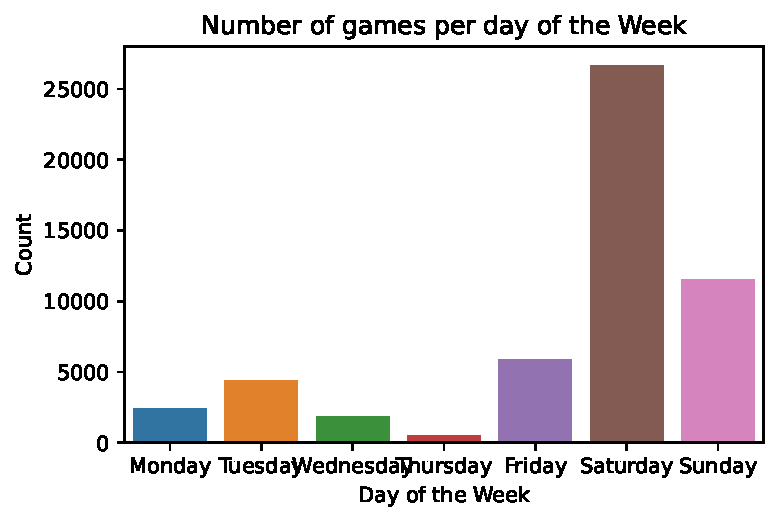
\includegraphics{Blog_post_files/figure-pdf/fig-count_day-output-1.pdf}

}

\caption{\label{fig-count_day}Number of games per day of the week}

\end{figure}

\begin{figure}

{\centering 

\begin{Shaded}
\begin{Highlighting}[]
\NormalTok{grouped\_week\_count\_division }\OperatorTok{=}\NormalTok{  time\_df.groupby([}\StringTok{\textquotesingle{}day\_of\_week\textquotesingle{}}\NormalTok{, }\StringTok{\textquotesingle{}division\textquotesingle{}}\NormalTok{]).count().reset\_index()}

\NormalTok{grouped\_week\_count\_division[}\StringTok{\textquotesingle{}day\_of\_week\textquotesingle{}}\NormalTok{] }\OperatorTok{=}\NormalTok{ pd.Categorical(grouped\_week\_count\_division[}\StringTok{\textquotesingle{}day\_of\_week\textquotesingle{}}\NormalTok{], categories}\OperatorTok{=}\NormalTok{ day\_categories)}
\NormalTok{grouped\_week\_count\_division.sort\_values(by }\OperatorTok{=} \StringTok{\textquotesingle{}day\_of\_week\textquotesingle{}}\NormalTok{, inplace }\OperatorTok{=} \VariableTok{True}\NormalTok{)}

\NormalTok{fig }\OperatorTok{=}\NormalTok{ px.bar(grouped\_week\_count\_division, y }\OperatorTok{=} \StringTok{\textquotesingle{}day\_of\_week\textquotesingle{}}\NormalTok{, x }\OperatorTok{=} \StringTok{\textquotesingle{}date\textquotesingle{}}\NormalTok{, color }\OperatorTok{=} \StringTok{\textquotesingle{}division\textquotesingle{}}\NormalTok{, barmode }\OperatorTok{=} \StringTok{\textquotesingle{}group\textquotesingle{}}\NormalTok{)}
\NormalTok{fig.show()}
\end{Highlighting}
\end{Shaded}

\begin{figure}

{\centering 

\begin{verbatim}
Unable to display output for mime type(s): text/html
\end{verbatim}

}

\caption{Number of games per day of week divided by League}

\end{figure}

\begin{figure}

{\centering 

\begin{verbatim}
Unable to display output for mime type(s): text/html
\end{verbatim}

}

\caption{\textbf{?(caption)}}

\end{figure}

}

\caption{\label{fig-day_median_attend_div}\textbf{?(caption)}}

\end{figure}

\hypertarget{time-of-day}{%
\subsection{Time of Day}\label{time-of-day}}

\begin{Shaded}
\begin{Highlighting}[]
\NormalTok{df\_grouped\_mean\_tod}\OperatorTok{=}\NormalTok{ time\_df.groupby(time\_df[}\StringTok{\textquotesingle{}date\_time\textquotesingle{}}\NormalTok{].dt.hour).mean()}
\NormalTok{df\_grouped\_median\_tod}\OperatorTok{=}\NormalTok{ time\_df.groupby(time\_df[}\StringTok{\textquotesingle{}date\_time\textquotesingle{}}\NormalTok{].dt.hour).median()}


\CommentTok{\# sns.lineplot(data = df\_grouped\_median\_tod, x = \textquotesingle{}date\_time\textquotesingle{}, y = \textquotesingle{}raw\_attendance\textquotesingle{}, markers = True, marker = "o" )}
\CommentTok{\# plt.title(\textquotesingle{}Attendance by Time of Day\textquotesingle{})}
\CommentTok{\# plt.xlabel(\textquotesingle{}Hour of the Day\textquotesingle{})}
\CommentTok{\# plt.ylabel(\textquotesingle{}Attendance\textquotesingle{})}
\CommentTok{\# plt.show()}
\end{Highlighting}
\end{Shaded}

Time and day of a match resulted in a similar situation as with day of
the week. In Figure~\ref{fig-attendance_time} there was sdips in
attendance at 3pm and 9pm however these were also the most attended
times for matches. 12pm and 11pm matches had the highest attendance on
average however had lower amount of games.

\begin{Shaded}
\begin{Highlighting}[]
\NormalTok{df\_grouped\_count }\OperatorTok{=}\NormalTok{ time\_df.groupby(time\_df[}\StringTok{\textquotesingle{}date\_time\textquotesingle{}}\NormalTok{].dt.hour).count()}
\CommentTok{\# print(df\_grouped\_count)}
\NormalTok{df\_grouped\_count }\OperatorTok{=}\NormalTok{ df\_grouped\_count[}\StringTok{\textquotesingle{}raw\_attendance\textquotesingle{}}\NormalTok{].reset\_index()}
\NormalTok{df\_grouped\_count[}\StringTok{\textquotesingle{}count\textquotesingle{}}\NormalTok{] }\OperatorTok{=}\NormalTok{ df\_grouped\_count[}\StringTok{\textquotesingle{}raw\_attendance\textquotesingle{}}\NormalTok{]}
\NormalTok{df\_grouped\_count }\OperatorTok{=}\NormalTok{ df\_grouped\_count[[}\StringTok{\textquotesingle{}date\_time\textquotesingle{}}\NormalTok{, }\StringTok{\textquotesingle{}count\textquotesingle{}}\NormalTok{]]}
\CommentTok{\# df\_grouped\_count= df\_grouped\_count.rename(columns = \{\textquotesingle{}date\textquotesingle{}:\textquotesingle{}count\textquotesingle{}\})}
\CommentTok{\# print(df\_grouped\_count)}

\NormalTok{df\_count\_atted }\OperatorTok{=}\NormalTok{ pd.merge(df\_grouped\_count, df\_grouped\_median\_tod, on }\OperatorTok{=} \StringTok{\textquotesingle{}date\_time\textquotesingle{}}\NormalTok{)}
\NormalTok{df\_count\_atted }\OperatorTok{=}\NormalTok{ df\_count\_atted.drop(columns}\OperatorTok{=}\NormalTok{ [}\StringTok{\textquotesingle{}capacity\_filled\textquotesingle{}}\NormalTok{])}
\NormalTok{df\_count\_atted.rename( columns }\OperatorTok{=}\NormalTok{ \{}\StringTok{\textquotesingle{}raw\_attendance\textquotesingle{}}\NormalTok{: }\StringTok{\textquotesingle{}Attendance\textquotesingle{}}\NormalTok{, }\StringTok{\textquotesingle{}count\textquotesingle{}}\NormalTok{: }\StringTok{"Number of Games"}\NormalTok{\}, inplace}\OperatorTok{=} \VariableTok{True}\NormalTok{)}
\CommentTok{\# print(df\_count\_atted)}
\NormalTok{melted\_count\_attend }\OperatorTok{=}\NormalTok{ pd.melt(df\_count\_atted, value\_vars}\OperatorTok{=}\NormalTok{[}\StringTok{\textquotesingle{}Number of Games\textquotesingle{}}\NormalTok{, }\StringTok{\textquotesingle{}Attendance\textquotesingle{}}\NormalTok{], id\_vars}\OperatorTok{=} \StringTok{\textquotesingle{}date\_time\textquotesingle{}}\NormalTok{)}
\CommentTok{\# print(melted\_count\_attend)}

\NormalTok{sns.lineplot(data }\OperatorTok{=}\NormalTok{ melted\_count\_attend, x }\OperatorTok{=} \StringTok{\textquotesingle{}date\_time\textquotesingle{}}\NormalTok{, y }\OperatorTok{=} \StringTok{\textquotesingle{}value\textquotesingle{}}\NormalTok{, hue }\OperatorTok{=} \StringTok{\textquotesingle{}variable\textquotesingle{}}\NormalTok{)}
\NormalTok{plt.title(}\StringTok{\textquotesingle{}Attendance and Game Count by Time of Day\textquotesingle{}}\NormalTok{)}
\NormalTok{plt.xlabel(}\StringTok{\textquotesingle{}Hour of the Day\textquotesingle{}}\NormalTok{)}

\NormalTok{plt.show()}
\end{Highlighting}
\end{Shaded}

\begin{figure}[H]

{\centering 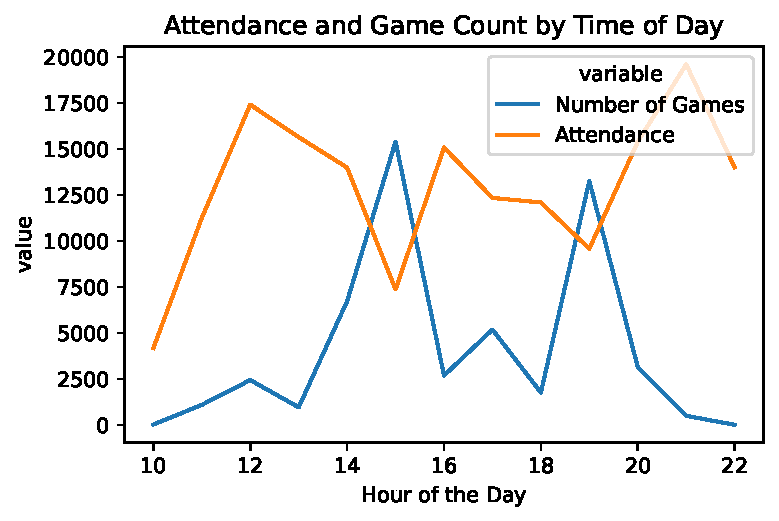
\includegraphics{Blog_post_files/figure-pdf/fig-attendance_time-output-1.pdf}

}

\caption{\label{fig-attendance_time}Attendance and Match count by time
of day}

\end{figure}

\hypertarget{calendar-date}{%
\subsection{Calendar Date}\label{calendar-date}}

The last aspect of when the match occured evaulated was what day of the
year a match occured. This is viewing trends during the calendar year to
see if there is any insight.

\begin{Shaded}
\begin{Highlighting}[]
\NormalTok{calendar\_plot\_data }\OperatorTok{=}\NormalTok{ total\_data}
\NormalTok{calendar\_plot\_data[}\StringTok{\textquotesingle{}month\_day\textquotesingle{}}\NormalTok{] }\OperatorTok{=}\NormalTok{ calendar\_plot\_data[}\StringTok{\textquotesingle{}date\_time\textquotesingle{}}\NormalTok{].dt.strftime(}\StringTok{\textquotesingle{}\%m{-}}\SpecialCharTok{\%d}\StringTok{\textquotesingle{}}\NormalTok{)}
\end{Highlighting}
\end{Shaded}

\hypertarget{trends-in-quanity-of-matches}{%
\subsection{Trends in Quanity of
Matches}\label{trends-in-quanity-of-matches}}

First before looking at the attendance its important to look and view
trends in when matches actually occur. In Figure~\ref{fig-cal_count},
there is a significantly low amount of games played from mid June to the
end of July. This can most likely be attributed to Europeans leagues
predominantly being on break during these months in relation to FIFA
internation break. On this break players typically return to their
national teams to play in international competitions and every four
years the world cup. Another significant period of time for number of
games is the Christmas holiday. Christmas has one of the lowest total
number of games occurring. However, December 26th or Boxing Day had the
most amount of games played for any day.

\begin{Shaded}
\begin{Highlighting}[]
\NormalTok{date\_of\_year }\OperatorTok{=}\NormalTok{ calendar\_plot\_data.groupby(}\StringTok{\textquotesingle{}month\_day\textquotesingle{}}\NormalTok{).count()}
\NormalTok{date\_of\_year[}\StringTok{\textquotesingle{}count\textquotesingle{}}\NormalTok{] }\OperatorTok{=}\NormalTok{ date\_of\_year[}\StringTok{\textquotesingle{}standard\_attend\textquotesingle{}}\NormalTok{]}
\NormalTok{date\_of\_year }\OperatorTok{=}\NormalTok{ date\_of\_year[}\StringTok{\textquotesingle{}count\textquotesingle{}}\NormalTok{].sort\_values().reset\_index()}
\CommentTok{\# print(date\_of\_year)}
\NormalTok{date\_of\_year[}\StringTok{\textquotesingle{}total\_date\textquotesingle{}}\NormalTok{] }\OperatorTok{=} \StringTok{\textquotesingle{}2024{-}\textquotesingle{}} \OperatorTok{+}\NormalTok{ date\_of\_year[}\StringTok{\textquotesingle{}month\_day\textquotesingle{}}\NormalTok{]}
\NormalTok{date\_of\_year[}\StringTok{\textquotesingle{}total\_date\textquotesingle{}}\NormalTok{]}\OperatorTok{=}\NormalTok{ pd.to\_datetime(date\_of\_year[}\StringTok{\textquotesingle{}total\_date\textquotesingle{}}\NormalTok{], }\BuiltInTok{format} \OperatorTok{=} \StringTok{"\%Y{-}\%m{-}}\SpecialCharTok{\%d}\StringTok{"}\NormalTok{)}
\NormalTok{events }\OperatorTok{=}\NormalTok{ pd.Series(date\_of\_year[}\StringTok{\textquotesingle{}count\textquotesingle{}}\NormalTok{].values.tolist(), index }\OperatorTok{=}\NormalTok{ date\_of\_year[}\StringTok{\textquotesingle{}total\_date\textquotesingle{}}\NormalTok{].values.tolist())}
\NormalTok{july.heatmap(dates }\OperatorTok{=}\NormalTok{ date\_of\_year[}\StringTok{\textquotesingle{}total\_date\textquotesingle{}}\NormalTok{], data }\OperatorTok{=}\NormalTok{ date\_of\_year[}\StringTok{\textquotesingle{}count\textquotesingle{}}\NormalTok{],  date\_label }\OperatorTok{=} \VariableTok{True}\NormalTok{, cmap }\OperatorTok{=} \StringTok{\textquotesingle{}RdYlBu\textquotesingle{}}\NormalTok{, fontsize }\OperatorTok{=}\DecValTok{10}\NormalTok{, weekday\_label}\OperatorTok{=}\VariableTok{False}\NormalTok{, year\_label}\OperatorTok{=} \VariableTok{False}\NormalTok{, title }\OperatorTok{=} \StringTok{\textquotesingle{}\# of Games per day 2010{-}2019\textquotesingle{}}\NormalTok{, colorbar}\OperatorTok{=} \VariableTok{True}\NormalTok{, dpi }\OperatorTok{=}\DecValTok{1200}\NormalTok{)}
\NormalTok{plt.show()}
\end{Highlighting}
\end{Shaded}

\begin{figure}[H]

{\centering 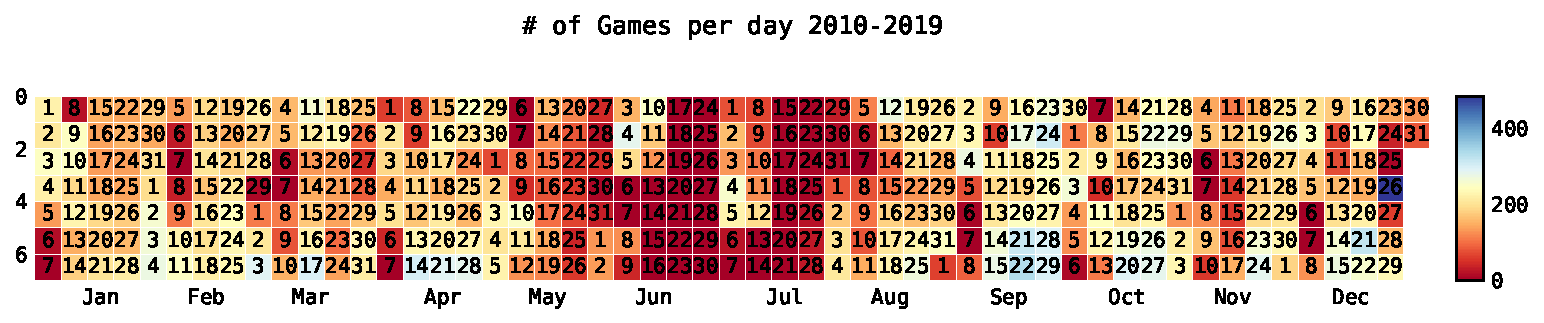
\includegraphics{Blog_post_files/figure-pdf/fig-cal_count-output-1.pdf}

}

\caption{\label{fig-cal_count}\textbf{?(caption)}}

\end{figure}

\hypertarget{trends-in-attedance-of-matches.}{%
\subsection{Trends in Attedance of
matches.}\label{trends-in-attedance-of-matches.}}

Now looking at the attendance for these matches based on their calendar
date some trends appear. First their is a grouping of higher than
average attendad matches in May. This can most likely be attributed to
the seasons across Europe are finishing. In turn these matches have
higher weight to them due to the ramifications of them. For teams at the
top and bottom of the standings, these matches have massive implications
for the club. They can result in the team being promoted (moved up a
league) or relegated (moved down a league) and access to European
competition. Additionally with holidays there is an affect on
attendance. First November 6th which is All Saint's day saw a decrease
in attendance on average. Christmas had lower than average attedance
while Boxing Day to New years eve had greater Attendance then what is
seen in December and January.

\begin{Shaded}
\begin{Highlighting}[]
\NormalTok{attend\_date }\OperatorTok{=}\NormalTok{ calendar\_plot\_data.groupby(}\StringTok{\textquotesingle{}month\_day\textquotesingle{}}\NormalTok{).mean()}
\NormalTok{attend\_date[}\StringTok{\textquotesingle{}count\textquotesingle{}}\NormalTok{] }\OperatorTok{=}\NormalTok{ attend\_date[}\StringTok{\textquotesingle{}standard\_attend\textquotesingle{}}\NormalTok{]}
\NormalTok{attend\_date }\OperatorTok{=}\NormalTok{ attend\_date[}\StringTok{\textquotesingle{}count\textquotesingle{}}\NormalTok{].sort\_values().reset\_index()}
\NormalTok{attend\_date[}\StringTok{\textquotesingle{}total\_date\textquotesingle{}}\NormalTok{] }\OperatorTok{=} \StringTok{\textquotesingle{}2024{-}\textquotesingle{}} \OperatorTok{+}\NormalTok{ attend\_date[}\StringTok{\textquotesingle{}month\_day\textquotesingle{}}\NormalTok{]}

\NormalTok{attend\_date[}\StringTok{\textquotesingle{}total\_date\textquotesingle{}}\NormalTok{] }\OperatorTok{=}\NormalTok{ pd.to\_datetime(attend\_date[}\StringTok{\textquotesingle{}total\_date\textquotesingle{}}\NormalTok{], }\BuiltInTok{format} \OperatorTok{=} \StringTok{"\%Y{-}\%m{-}}\SpecialCharTok{\%d}\StringTok{"}\NormalTok{)}
\NormalTok{events }\OperatorTok{=}\NormalTok{ pd.Series(attend\_date[}\StringTok{\textquotesingle{}count\textquotesingle{}}\NormalTok{].values.tolist(), index }\OperatorTok{=}\NormalTok{ attend\_date[}\StringTok{\textquotesingle{}total\_date\textquotesingle{}}\NormalTok{].values.tolist())}
\NormalTok{july.heatmap(dates }\OperatorTok{=}\NormalTok{ attend\_date[}\StringTok{\textquotesingle{}total\_date\textquotesingle{}}\NormalTok{], data }\OperatorTok{=}\NormalTok{ attend\_date[}\StringTok{\textquotesingle{}count\textquotesingle{}}\NormalTok{],  cmap}\OperatorTok{=}\StringTok{\textquotesingle{}RdYlBu\textquotesingle{}}\NormalTok{, date\_label }\OperatorTok{=} \VariableTok{True}\NormalTok{, fontsize }\OperatorTok{=}\DecValTok{10}\NormalTok{, weekday\_label}\OperatorTok{=}\VariableTok{False}\NormalTok{, year\_label}\OperatorTok{=} \VariableTok{False}\NormalTok{, title }\OperatorTok{=} \StringTok{\textquotesingle{}Avg Attendance per day Standardized 2010{-}2019\textquotesingle{}}\NormalTok{, colorbar}\OperatorTok{=} \VariableTok{True}\NormalTok{, dpi }\OperatorTok{=}\DecValTok{1200}\NormalTok{)}
\NormalTok{plt.show()}
\end{Highlighting}
\end{Shaded}

\begin{figure}[H]

{\centering 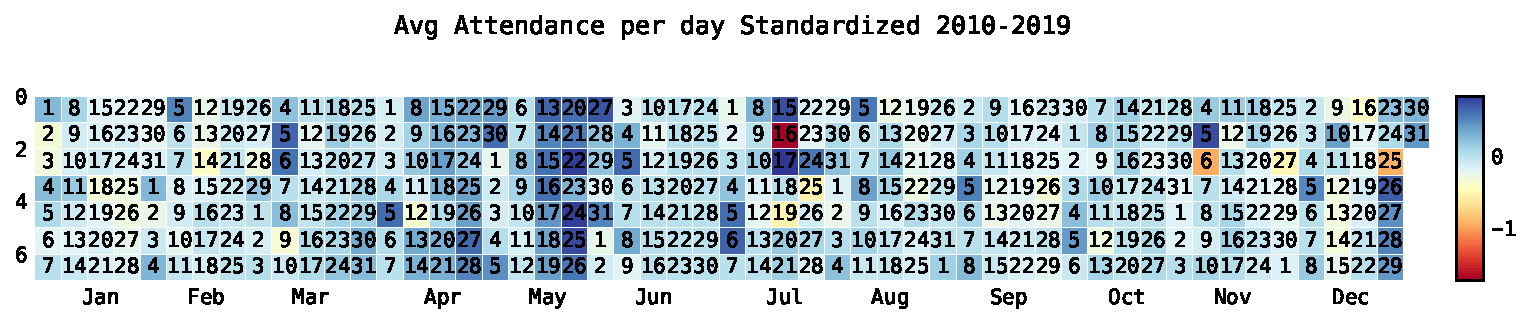
\includegraphics{Blog_post_files/figure-pdf/fig-cal_attend-output-1.pdf}

}

\caption{\label{fig-cal_attend}\textbf{?(caption)}}

\end{figure}

\hypertarget{away-team-impact}{%
\section{Away Team Impact}\label{away-team-impact}}

\begin{Shaded}
\begin{Highlighting}[]
\NormalTok{away\_team\_impact }\OperatorTok{=}\NormalTok{ total\_data.groupby([}\StringTok{\textquotesingle{}away\_team\textquotesingle{}}\NormalTok{, }\StringTok{\textquotesingle{}division\textquotesingle{}}\NormalTok{])[}\StringTok{\textquotesingle{}standard\_attend\textquotesingle{}}\NormalTok{].mean().reset\_index()}


\CommentTok{\# away\_team\_impact = away\_team\_impact[away\_team\_impact[\textquotesingle{}division\textquotesingle{}].isin([\textquotesingle{}E3\textquotesingle{}, \textquotesingle{}E1\textquotesingle{}, \textquotesingle{}E2\textquotesingle{}])]}
\NormalTok{div\_dict }\OperatorTok{=}\NormalTok{ \{}\StringTok{\textquotesingle{}D1\textquotesingle{}}\NormalTok{:}\StringTok{\textquotesingle{}Bundesliga\textquotesingle{}}\NormalTok{, }\StringTok{\textquotesingle{}D2\textquotesingle{}}\NormalTok{: }\StringTok{\textquotesingle{}2. Bundesliga\textquotesingle{}}\NormalTok{, }\StringTok{\textquotesingle{}E0\textquotesingle{}}\NormalTok{:}\StringTok{\textquotesingle{}Premier League\textquotesingle{}}\NormalTok{, }\StringTok{\textquotesingle{}E1\textquotesingle{}}\NormalTok{:}\StringTok{\textquotesingle{}Championship\textquotesingle{}}\NormalTok{, }
            \StringTok{\textquotesingle{}E2\textquotesingle{}}\NormalTok{:}\StringTok{\textquotesingle{}League 1\textquotesingle{}}\NormalTok{, }\StringTok{\textquotesingle{}E3\textquotesingle{}}\NormalTok{:}\StringTok{\textquotesingle{}Leauge 2\textquotesingle{}}\NormalTok{,}\StringTok{\textquotesingle{}SP1\textquotesingle{}}\NormalTok{:}\StringTok{\textquotesingle{}La Liga Primera\textquotesingle{}}\NormalTok{, }\StringTok{\textquotesingle{}SP2\textquotesingle{}}\NormalTok{:}\StringTok{\textquotesingle{}La Liga Segunda\textquotesingle{}}\NormalTok{,}
              \StringTok{\textquotesingle{}B1\textquotesingle{}}\NormalTok{:}\StringTok{\textquotesingle{}Jupiler League\textquotesingle{}}\NormalTok{, }\StringTok{\textquotesingle{}F1\textquotesingle{}}\NormalTok{:}\StringTok{\textquotesingle{}Ligue 1\textquotesingle{}}\NormalTok{,}\StringTok{\textquotesingle{}F2\textquotesingle{}}\NormalTok{:}\StringTok{\textquotesingle{}Ligue 2\textquotesingle{}}\NormalTok{,}\StringTok{\textquotesingle{}I1\textquotesingle{}}\NormalTok{:}\StringTok{\textquotesingle{}Serie A\textquotesingle{}}\NormalTok{,}\StringTok{\textquotesingle{}I2\textquotesingle{}}\NormalTok{:}\StringTok{\textquotesingle{}Seire B\textquotesingle{}}\NormalTok{, }
              \StringTok{\textquotesingle{}SC0\textquotesingle{}}\NormalTok{:}\StringTok{\textquotesingle{}Scotish Premier League\textquotesingle{}}\NormalTok{, }\StringTok{\textquotesingle{}SC1\textquotesingle{}}\NormalTok{:}\StringTok{\textquotesingle{}Scotish Division 1\textquotesingle{}}\NormalTok{, }\StringTok{\textquotesingle{}T1\textquotesingle{}}\NormalTok{:}\StringTok{\textquotesingle{}Fubol Ligi 1\textquotesingle{}}\NormalTok{, }\StringTok{\textquotesingle{}P1\textquotesingle{}}\NormalTok{: }\StringTok{\textquotesingle{}Liga 1\textquotesingle{}}\NormalTok{\}}
\NormalTok{divisions\_list }\OperatorTok{=}\NormalTok{[}\StringTok{\textquotesingle{}D1\textquotesingle{}}\NormalTok{, }\StringTok{\textquotesingle{}D2\textquotesingle{}}\NormalTok{, }\StringTok{\textquotesingle{}E0\textquotesingle{}}\NormalTok{, }\StringTok{\textquotesingle{}E1\textquotesingle{}}\NormalTok{, }\StringTok{\textquotesingle{}E2\textquotesingle{}}\NormalTok{, }\StringTok{\textquotesingle{}E3\textquotesingle{}}\NormalTok{, }\StringTok{\textquotesingle{}SP1\textquotesingle{}}\NormalTok{ ,}\StringTok{\textquotesingle{}SP2\textquotesingle{}}\NormalTok{, }\StringTok{\textquotesingle{}B1\textquotesingle{}}\NormalTok{, }\StringTok{\textquotesingle{}F1\textquotesingle{}}\NormalTok{, }\StringTok{\textquotesingle{}F2\textquotesingle{}}\NormalTok{, }\StringTok{\textquotesingle{}I1\textquotesingle{}}\NormalTok{, }\StringTok{\textquotesingle{}I2\textquotesingle{}}\NormalTok{, }\StringTok{\textquotesingle{}SC0\textquotesingle{}}\NormalTok{, }\StringTok{\textquotesingle{}SC1\textquotesingle{}}\NormalTok{, }\StringTok{\textquotesingle{}T1\textquotesingle{}}\NormalTok{, }\StringTok{\textquotesingle{}P1\textquotesingle{}}\NormalTok{]}

\NormalTok{away\_team\_impact }\OperatorTok{=}\NormalTok{ away\_team\_impact[[}\StringTok{\textquotesingle{}away\_team\textquotesingle{}}\NormalTok{, }\StringTok{\textquotesingle{}division\textquotesingle{}}\NormalTok{, }\StringTok{\textquotesingle{}standard\_attend\textquotesingle{}}\NormalTok{]]}
\CommentTok{\# print(away\_team\_impact)}
\NormalTok{initial\_graph\_df }\OperatorTok{=}\NormalTok{ pd.DataFrame(columns }\OperatorTok{=}\NormalTok{ [}\StringTok{\textquotesingle{}away\_team\textquotesingle{}}\NormalTok{, }\StringTok{\textquotesingle{}division\textquotesingle{}}\NormalTok{, }\StringTok{\textquotesingle{}standard\_attend\textquotesingle{}}\NormalTok{])}

\ControlFlowTok{for}\NormalTok{ i }\KeywordTok{in}\NormalTok{ divisions\_list:}
\NormalTok{        temp\_impact\_df }\OperatorTok{=}\NormalTok{ away\_team\_impact[away\_team\_impact[}\StringTok{\textquotesingle{}division\textquotesingle{}}\NormalTok{] }\OperatorTok{==}\NormalTok{ i].sort\_values(}\StringTok{\textquotesingle{}standard\_attend\textquotesingle{}}\NormalTok{,ascending }\OperatorTok{=} \VariableTok{False}\NormalTok{).head(}\DecValTok{3}\NormalTok{)}
\NormalTok{        initial\_graph\_df }\OperatorTok{=}\NormalTok{ pd.concat([initial\_graph\_df, temp\_impact\_df], axis }\OperatorTok{=} \DecValTok{0}\NormalTok{)}


\CommentTok{\# fig = go.Figure(px.bar(away\_team\_impact, y= \textquotesingle{}away\_team\textquotesingle{}, x = \textquotesingle{}standard\_attend\textquotesingle{}, color = \textquotesingle{}division\textquotesingle{}))}

\NormalTok{app }\OperatorTok{=}\NormalTok{ JupyterDash(}\VariableTok{\_\_name\_\_}\NormalTok{)}
\NormalTok{app.layout }\OperatorTok{=}\NormalTok{ html.Div(}\BuiltInTok{id} \OperatorTok{=} \StringTok{\textquotesingle{}parent\textquotesingle{}}\NormalTok{, children }\OperatorTok{=}\NormalTok{ [}
\NormalTok{    html.H1(}\BuiltInTok{id} \OperatorTok{=} \StringTok{\textquotesingle{}H1\textquotesingle{}}\NormalTok{, children }\OperatorTok{=} \StringTok{\textquotesingle{}Away Team Impact\textquotesingle{}}\NormalTok{),}
\NormalTok{    dcc.Slider(}\DecValTok{0}\NormalTok{,}\DecValTok{20}\NormalTok{,}\DecValTok{1}\NormalTok{, value }\OperatorTok{=}\DecValTok{3}\NormalTok{,}\BuiltInTok{id} \OperatorTok{=} \StringTok{\textquotesingle{}slider\textquotesingle{}}\NormalTok{),}
\NormalTok{    dcc.Dropdown(}\BuiltInTok{id} \OperatorTok{=} \StringTok{\textquotesingle{}dropdown\textquotesingle{}}\NormalTok{, }
\NormalTok{                 options }\OperatorTok{=}\NormalTok{ [}
\NormalTok{                \{}\StringTok{\textquotesingle{}label\textquotesingle{}}\NormalTok{: }\StringTok{\textquotesingle{}Bundesliga\textquotesingle{}}\NormalTok{, }\StringTok{\textquotesingle{}value\textquotesingle{}}\NormalTok{:}\StringTok{\textquotesingle{}D1\textquotesingle{}}\NormalTok{\},}
\NormalTok{                \{}\StringTok{\textquotesingle{}label\textquotesingle{}}\NormalTok{: }\StringTok{\textquotesingle{}2. Bundesliga\textquotesingle{}}\NormalTok{, }\StringTok{\textquotesingle{}value\textquotesingle{}}\NormalTok{:}\StringTok{\textquotesingle{}D2\textquotesingle{}}\NormalTok{\},}
\NormalTok{                \{}\StringTok{\textquotesingle{}label\textquotesingle{}}\NormalTok{: }\StringTok{\textquotesingle{}Premier League\textquotesingle{}}\NormalTok{, }\StringTok{\textquotesingle{}value\textquotesingle{}}\NormalTok{:}\StringTok{\textquotesingle{}E0\textquotesingle{}}\NormalTok{\},}
\NormalTok{                \{}\StringTok{\textquotesingle{}label\textquotesingle{}}\NormalTok{: }\StringTok{\textquotesingle{}Championship\textquotesingle{}}\NormalTok{, }\StringTok{\textquotesingle{}value\textquotesingle{}}\NormalTok{:}\StringTok{\textquotesingle{}E1\textquotesingle{}}\NormalTok{\},}
\NormalTok{                \{}\StringTok{\textquotesingle{}label\textquotesingle{}}\NormalTok{: }\StringTok{\textquotesingle{}League 1\textquotesingle{}}\NormalTok{, }\StringTok{\textquotesingle{}value\textquotesingle{}}\NormalTok{:}\StringTok{\textquotesingle{}E2\textquotesingle{}}\NormalTok{\},}
\NormalTok{                \{}\StringTok{\textquotesingle{}label\textquotesingle{}}\NormalTok{: }\StringTok{\textquotesingle{}Leauge 2\textquotesingle{}}\NormalTok{, }\StringTok{\textquotesingle{}value\textquotesingle{}}\NormalTok{:}\StringTok{\textquotesingle{}E3\textquotesingle{}}\NormalTok{\},}
\NormalTok{                \{}\StringTok{\textquotesingle{}label\textquotesingle{}}\NormalTok{: }\StringTok{\textquotesingle{}La Liga Primera\textquotesingle{}}\NormalTok{, }\StringTok{\textquotesingle{}value\textquotesingle{}}\NormalTok{:}\StringTok{\textquotesingle{}SP1\textquotesingle{}}\NormalTok{\},}
\NormalTok{                \{}\StringTok{\textquotesingle{}label\textquotesingle{}}\NormalTok{: }\StringTok{\textquotesingle{}La Liga Segunda\textquotesingle{}}\NormalTok{, }\StringTok{\textquotesingle{}value\textquotesingle{}}\NormalTok{:}\StringTok{\textquotesingle{}SP2\textquotesingle{}}\NormalTok{\},}
\NormalTok{                \{}\StringTok{\textquotesingle{}label\textquotesingle{}}\NormalTok{: }\StringTok{\textquotesingle{}Jupiler League\textquotesingle{}}\NormalTok{, }\StringTok{\textquotesingle{}value\textquotesingle{}}\NormalTok{:}\StringTok{\textquotesingle{}B1\textquotesingle{}}\NormalTok{\},}
\NormalTok{                \{}\StringTok{\textquotesingle{}label\textquotesingle{}}\NormalTok{: }\StringTok{\textquotesingle{}Ligue 1\textquotesingle{}}\NormalTok{, }\StringTok{\textquotesingle{}value\textquotesingle{}}\NormalTok{:}\StringTok{\textquotesingle{}F1\textquotesingle{}}\NormalTok{\},}
\NormalTok{                \{}\StringTok{\textquotesingle{}label\textquotesingle{}}\NormalTok{: }\StringTok{\textquotesingle{}Ligue 2\textquotesingle{}}\NormalTok{, }\StringTok{\textquotesingle{}value\textquotesingle{}}\NormalTok{:}\StringTok{\textquotesingle{}F2\textquotesingle{}}\NormalTok{\},}
\NormalTok{                \{}\StringTok{\textquotesingle{}label\textquotesingle{}}\NormalTok{: }\StringTok{\textquotesingle{}Serie A\textquotesingle{}}\NormalTok{, }\StringTok{\textquotesingle{}value\textquotesingle{}}\NormalTok{:}\StringTok{\textquotesingle{}I1\textquotesingle{}}\NormalTok{\},}
\NormalTok{                \{}\StringTok{\textquotesingle{}label\textquotesingle{}}\NormalTok{: }\StringTok{\textquotesingle{}Serie B\textquotesingle{}}\NormalTok{, }\StringTok{\textquotesingle{}value\textquotesingle{}}\NormalTok{:}\StringTok{\textquotesingle{}I2\textquotesingle{}}\NormalTok{\},}
\NormalTok{                \{}\StringTok{\textquotesingle{}label\textquotesingle{}}\NormalTok{: }\StringTok{\textquotesingle{}Scotish Premier League\textquotesingle{}}\NormalTok{, }\StringTok{\textquotesingle{}value\textquotesingle{}}\NormalTok{:}\StringTok{\textquotesingle{}SC0\textquotesingle{}}\NormalTok{\},}
\NormalTok{                \{}\StringTok{\textquotesingle{}label\textquotesingle{}}\NormalTok{: }\StringTok{\textquotesingle{}Scotish Division 1\textquotesingle{}}\NormalTok{, }\StringTok{\textquotesingle{}value\textquotesingle{}}\NormalTok{:}\StringTok{\textquotesingle{}SC1\textquotesingle{}}\NormalTok{\},}
\NormalTok{                \{}\StringTok{\textquotesingle{}label\textquotesingle{}}\NormalTok{: }\StringTok{\textquotesingle{}Fubol Ligi 1\textquotesingle{}}\NormalTok{, }\StringTok{\textquotesingle{}value\textquotesingle{}}\NormalTok{:}\StringTok{\textquotesingle{}T1\textquotesingle{}}\NormalTok{\},}
\NormalTok{                \{}\StringTok{\textquotesingle{}label\textquotesingle{}}\NormalTok{: }\StringTok{\textquotesingle{}Liga 1\textquotesingle{}}\NormalTok{, }\StringTok{\textquotesingle{}value\textquotesingle{}}\NormalTok{:}\StringTok{\textquotesingle{}P1\textquotesingle{}}\NormalTok{\}}


\NormalTok{                 ], value }\OperatorTok{=}\NormalTok{ [}\StringTok{\textquotesingle{}D1\textquotesingle{}}\NormalTok{, }\StringTok{\textquotesingle{}D2\textquotesingle{}}\NormalTok{, }\StringTok{\textquotesingle{}E0\textquotesingle{}}\NormalTok{, }\StringTok{\textquotesingle{}E1\textquotesingle{}}\NormalTok{, }\StringTok{\textquotesingle{}E2\textquotesingle{}}\NormalTok{, }\StringTok{\textquotesingle{}E3\textquotesingle{}}\NormalTok{, }\StringTok{\textquotesingle{}SP1\textquotesingle{}}\NormalTok{ ,}\StringTok{\textquotesingle{}SP2\textquotesingle{}}\NormalTok{, }\StringTok{\textquotesingle{}B1\textquotesingle{}}\NormalTok{, }\StringTok{\textquotesingle{}F1\textquotesingle{}}\NormalTok{, }\StringTok{\textquotesingle{}F2\textquotesingle{}}\NormalTok{, }\StringTok{\textquotesingle{}I1\textquotesingle{}}\NormalTok{, }\StringTok{\textquotesingle{}I2\textquotesingle{}}\NormalTok{, }\StringTok{\textquotesingle{}SC0\textquotesingle{}}\NormalTok{, }\StringTok{\textquotesingle{}SC1\textquotesingle{}}\NormalTok{, }\StringTok{\textquotesingle{}T1\textquotesingle{}}\NormalTok{, }\StringTok{\textquotesingle{}P1\textquotesingle{}}\NormalTok{],}
\NormalTok{                 multi }\OperatorTok{=} \VariableTok{True}\NormalTok{),}
\NormalTok{    dcc.Graph(}\BuiltInTok{id} \OperatorTok{=} \StringTok{\textquotesingle{}bar\_plot\textquotesingle{}}\NormalTok{, figure}\OperatorTok{=}\NormalTok{px.bar(initial\_graph\_df, x}\OperatorTok{=}\StringTok{\textquotesingle{}away\_team\textquotesingle{}}\NormalTok{, y}\OperatorTok{=}\StringTok{\textquotesingle{}standard\_attend\textquotesingle{}}\NormalTok{, color}\OperatorTok{=}\StringTok{\textquotesingle{}division\textquotesingle{}}\NormalTok{))}
\NormalTok{])}

\AttributeTok{@app.callback}\NormalTok{(}
\NormalTok{    Output(}\StringTok{"bar\_plot"}\NormalTok{, }\StringTok{"figure"}\NormalTok{), }
\NormalTok{    [Input(}\StringTok{"dropdown"}\NormalTok{, }\StringTok{"value"}\NormalTok{),}
\NormalTok{     Input(}\StringTok{\textquotesingle{}slider\textquotesingle{}}\NormalTok{, }\StringTok{\textquotesingle{}value\textquotesingle{}}\NormalTok{)]}
\NormalTok{    )}
\KeywordTok{def}\NormalTok{ update\_graph(drop\_value, slider\_value):}
    \CommentTok{\# print(value)}
\NormalTok{    df }\OperatorTok{=}\NormalTok{ away\_team\_impact}

    

\NormalTok{    df }\OperatorTok{=}\NormalTok{ df[df[}\StringTok{\textquotesingle{}division\textquotesingle{}}\NormalTok{].isin(}\BuiltInTok{list}\NormalTok{(drop\_value))]}
\NormalTok{    graph\_df }\OperatorTok{=}\NormalTok{ pd.DataFrame(columns }\OperatorTok{=}\NormalTok{ [}\StringTok{\textquotesingle{}away\_team\textquotesingle{}}\NormalTok{, }\StringTok{\textquotesingle{}division\textquotesingle{}}\NormalTok{, }\StringTok{\textquotesingle{}standard\_attend\textquotesingle{}}\NormalTok{])}
    \ControlFlowTok{for}\NormalTok{ i }\KeywordTok{in}\NormalTok{ drop\_value:}
\NormalTok{        temp\_impact\_df }\OperatorTok{=}\NormalTok{ df[df[}\StringTok{\textquotesingle{}division\textquotesingle{}}\NormalTok{] }\OperatorTok{==}\NormalTok{ i].sort\_values(}\StringTok{\textquotesingle{}standard\_attend\textquotesingle{}}\NormalTok{,ascending }\OperatorTok{=} \VariableTok{False}\NormalTok{).head(slider\_value)}
\NormalTok{        graph\_df }\OperatorTok{=}\NormalTok{ pd.concat([graph\_df, temp\_impact\_df], axis }\OperatorTok{=} \DecValTok{0}\NormalTok{)}
\NormalTok{    graph\_df }\OperatorTok{=}\NormalTok{ graph\_df.reset\_index().drop(columns }\OperatorTok{=}\NormalTok{ [}\StringTok{\textquotesingle{}index\textquotesingle{}}\NormalTok{])}
\NormalTok{    fig }\OperatorTok{=}\NormalTok{ px.bar(graph\_df, x}\OperatorTok{=} \StringTok{\textquotesingle{}away\_team\textquotesingle{}}\NormalTok{, y}\OperatorTok{=} \StringTok{\textquotesingle{}standard\_attend\textquotesingle{}}\NormalTok{, color }\OperatorTok{=} \StringTok{\textquotesingle{}division\textquotesingle{}}\NormalTok{)}
    \ControlFlowTok{return}\NormalTok{ fig}
\ControlFlowTok{if} \VariableTok{\_\_name\_\_} \OperatorTok{==} \StringTok{\textquotesingle{}\_\_main\_\_\textquotesingle{}}\NormalTok{:}
\NormalTok{    app.run\_server(mode}\OperatorTok{=}\StringTok{\textquotesingle{}inline\textquotesingle{}}\NormalTok{)}
\end{Highlighting}
\end{Shaded}

\begin{verbatim}
Dash is running on http://127.0.0.1:8050/
\end{verbatim}

\begin{verbatim}
<IPython.lib.display.IFrame at 0x27ca99075b0>
\end{verbatim}



\end{document}
